% Two-page summary: can GIPL 2.0 ground temperatures be trusted?
% Build: see the header of scripts/03_report/build_gipl_trust.sh (xelatex, Liberation Sans).
% Figures: scripts/03_report/gipl_trust_figures.py -> docs/figures/gipl_trust_*.pdf
\documentclass[10pt]{article}
\usepackage[letterpaper, top=0.45in, bottom=0.4in, left=0.6in, right=0.6in]{geometry}
\usepackage{fontspec}
\setmainfont{Liberation Sans}
\usepackage{xcolor}
\usepackage{graphicx}
\usepackage{enumitem}
\usepackage{microtype}
\usepackage[hidelinks]{hyperref}

\definecolor{ink}{HTML}{0B0B0B}
\definecolor{ink2}{HTML}{52514E}
\definecolor{accent}{HTML}{C2410C}
\definecolor{boxbg}{HTML}{F3F2EE}
\definecolor{rule}{HTML}{C3C2B7}

\renewcommand\normalsize{\fontsize{8.9}{11.0}\selectfont}
\renewcommand\small{\fontsize{7.6}{9.3}\selectfont}
\renewcommand\footnotesize{\fontsize{6.7}{8.2}\selectfont}
\pagestyle{empty}
\setlength{\parindent}{0pt}
\raggedright
\setlength{\parskip}{3pt}
\color{ink}
\setlist{nosep, leftmargin=1.1em, topsep=1pt, itemsep=1pt}

% section heading: number in accent colour, title in bold
\newcommand{\problem}[2]{%
  \par\vspace{6pt}{\fontsize{11}{13}\selectfont\bfseries\textcolor{accent}{#1}\hspace{0.45em}#2\par}%
  \vspace{1pt}{\color{rule}\hrule height 0.5pt}\vspace{3pt}}
\newcommand{\fig}[2]{\par\vspace{2pt}\noindent\includegraphics[width=#1]{#2}\par}
\newcommand{\figcap}[1]{{\small\color{ink2}#1\par}\vspace{2pt}}

\begin{document}
\normalsize

{\small\color{ink2}\MakeUppercase{Data quality summary}\hfill October 2026\par}
\vspace{3pt}
{\fontsize{17}{20}\selectfont\bfseries Can we trust the GIPL 2.0 permafrost projections?\par}
\vspace{2pt}
{\color{ink2}GIPL 2.0 ground temperature projections for Alaska (SNAP, University of Alaska Fairbanks): 1\,km,
files labelled 2021--2120, three climate inputs (5-model average, GFDL-CM3, NCAR-CCSM4), RCP 4.5 and 8.5.\par}
\vspace{5pt}

\noindent\colorbox{boxbg}{\parbox{\dimexpr\linewidth-2\fboxsep}{\raggedright\vspace{2pt}%
We compared GIPL 2.0 with a satellite-based product (ESA CCI Permafrost), 90 boreholes, about 2,800 CUSP field sites
and the climate data that drove it. We found four problems:
\begin{enumerate}[label=\textbf{\textcolor{accent}{\arabic*}}, leftmargin=1.2em, topsep=1pt]
  \item \textbf{Mislabelled years.} Every file is labelled 20 years late: ``2021'' holds the climate of 2001.
  \item \textbf{Stuck cells.} Across 46,000\,km², mostly in the Interior, the ground from 1\,m down never warms.
  \item \textbf{Right on average, not cell by cell.} Single cells differ from other estimates by up to about 2\,°C.
  \item \textbf{An unexplained start, and two unexplained runs} (NCAR-CCSM4).
\end{enumerate}
\vspace{1pt}
Problems 1 and 3 can be worked around. Problems 2 and 4 sit in the delivered data, and the run is undocumented, so
their causes cannot be identified.\vspace{2pt}}}

\problem{1}{Mislabelled years}
GIPL turns monthly air temperature and snow into ground temperature, so its warm and cold years should follow those of
the climate data that drove it. As labelled, they do not (Fig.~1a). Shifted by 20 years, they line up almost exactly
(Fig.~1b): for GFDL-CM3, the year-to-year match is 0.94--0.95 in every cell, and a separately downscaled version of the
same climate model confirms the shift. Read on the right years:
\begin{itemize}
  \item The data cover \textbf{2001--2100}, not 2021--2120. The first 15 years are \textbf{observed weather
    (2001--2015)}, the same in every run; the projections start in 2016. One run (GFDL-CM3, RCP 8.5) is shifted 19
    years, and its last file repeats the one before.
  \item GIPL was driven by SNAP's 2\,km downscaled climate, the same product we compare it with.
  \item Taken at face value, the labels set GIPL against the wrong years: in our first audit, that made GIPL look
    1--2\,°C too cold and its warming out of step with the air. Neither holds on the right years.
\end{itemize}
\fig{\linewidth}{figures/gipl_trust_1_years.pdf}
\figcap{\textbf{Figure 1.} Year-to-year change of GIPL's ground surface temperature (GFDL-CM3, RCP 4.5, statewide
median) next to the air temperature that drove it. (a) As labelled. (b) GIPL moved 20 years earlier; dashed: observed
air. r: median correlation per cell.}

\problem{2}{Stuck cells: ground that never warms}
In 1,172 patches covering \textbf{46,000\,km² (4.6\,\% of Alaska's permafrost area)}, GIPL's temperature at 1\,m
changes by less than 0.1\,°C over the whole run, under every climate model and scenario. \textbf{88\,\% of this area is
in the Interior, where it covers 10\,\% of the permafrost area, or 19\,\% with the 2\,km border.}
The ground temperature is also stuck at every deeper level we checked (2, 3 and 5\,m), and 0.5\,m warms only 0.4\,°C over the
century (about 5\,°C elsewhere). Each cell holds its own fixed value (−5 to −1\,°C at 1\,m). Yet their surface warms
\emph{faster} than nearby cells' (1.5--3.5\,°C warmer by the end of the century), and cells within 2\,km are partly
affected. Satellite data show nothing unusual there, and soil and land-cover maps do not explain the pattern.
\fig{\linewidth}{figures/gipl_trust_2_stuck.pdf}
\figcap{\textbf{Figure 2.} (a) Cells where 1\,m temperature changes by < 0.1\,°C over the run. (b, c) A stuck and a
normal cell 4\,km apart (5-model average, RCP 8.5; years shifted as in problem 1; air: observed to 2015, then
projected).}

\newpage

\problem{3}{Right on average, not cell by cell}
On the right years, three independent checks agree that GIPL's temperatures are about right on average:
\begin{itemize}
  \item \textbf{Satellite-based product (ESA CCI)}, 2004--2015 (both driven by observed weather): within 0.2\,°C at
    1 and 2\,m, and 0.9\,°C warmer at the ground surface (statewide median).
  \item \textbf{90 monitoring boreholes}, same years: median error −0.3, −0.5 and −0.05\,°C at the surface, 1\,m
    and 2\,m; ESA CCI −0.5, +0.3 and +0.4\,°C (Fig.~3b).
  \item \textbf{About 2,800 CUSP field sites}, where crews recorded whether permafrost was present: at 1\,m, the
    temperature that best separates the two groups is −0.2\,°C in GIPL (ESA CCI: +1.4\,°C; Fig.~3c).
\end{itemize}
But single cells differ from ESA CCI by −1.5 to +1.9\,°C (middle 80\,\%, 1\,m), in a clear regional pattern
(Fig.~3a). Where ESA CCI puts the ground at +1 to +3\,°C, GIPL is 1.4--2.1\,°C colder: it holds thawing ground near
0\,°C while the ice melts, so small errors decide whether a cell reads frozen or thawed.
\fig{\linewidth}{figures/gipl_trust_3_levels.pdf}
\figcap{\textbf{Figure 3.} (a) GIPL minus ESA CCI at 1\,m, 2004--2015 (RCP 8.5). (b) Measured vs.\ dataset temperature,
same years. (c) GIPL's 1\,m temperature at field sites with and without permafrost.}

\problem{4}{An unexplained start, and two unexplained runs}
\noindent\begin{minipage}[t]{0.505\linewidth}
\vspace{0pt}\raggedright
\begin{itemize}
  \item \textbf{A three-year start-up.} At 1\,m the statewide median climbs 1.8\,°C from 2001 to 2003 (Fig.~4a);
    real ground does not warm that fast. 2001--2003 should not be used.
  \item \textbf{Mixed-up starting points.} The two scenarios start up to 1.7\,°C apart although their weather is
    the same (observed) until 2015, while four of the six runs start from identical values in every cell.
  \item \textbf{NCAR-CCSM4.} Both runs match no climate data we could find (SNAP's CCSM4 at 2\,km or 771\,m, a
    separately downscaled CCSM4, observations), and their surface spikes 3.6--5.1\,°C in 2003 (Fig.~4b).
\end{itemize}
\end{minipage}\hfill
\begin{minipage}[t]{0.475\linewidth}
\vspace{0pt}
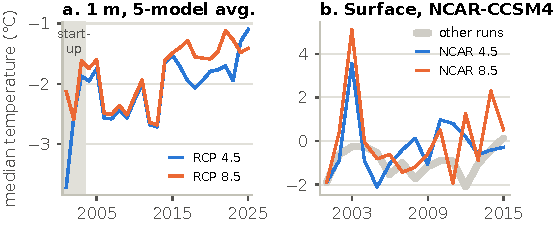
\includegraphics[width=\linewidth]{figures/gipl_trust_4_runs.pdf}
\figcap{\textbf{Figure 4.} Statewide median of permafrost cells (stuck cells excluded), climate years. (a) Start-up
at 1\,m. (b) NCAR-CCSM4's surface against the other runs.}
\end{minipage}

\vspace{2pt}
\noindent\colorbox{boxbg}{\parbox{\dimexpr\linewidth-2\fboxsep}{\raggedright\vspace{3pt}%
\textbf{What still holds.} GIPL's spatial pattern is sound: it ranks colder and warmer places as well as ESA CCI does
at the field sites. Its warming follows the scenarios, damped: over 2036--2070 its surface warms 0.3 (RCP 4.5) and
0.7\,°C (RCP 8.5) per decade, against 0.3 and 0.9\,°C for the projected air, and less at depth. Snow and soil can
explain such a lag, but the recent record points the other way: over 2003--2023 the satellite-based ground surface
warmed faster than the observed air (0.62 vs 0.37\,°C per decade).\par\vspace{4pt}
\textbf{If GIPL 2.0 is used,} four steps follow from these findings: read every file as the climate of the year in
its name minus 20 (minus 19 for GFDL-CM3, RCP 8.5); skip 2001--2003; mask the stuck cells and their 2\,km border
(about 9\,\% of Alaska's permafrost area); and treat single-cell values as uncertain by up to about 2\,°C. The
NCAR-CCSM4 runs need extra caution. The causes of problems 2 and 4 cannot be
identified: no documentation exists for this 1\,km run, including its climate inputs, starting conditions, and soil and
snow settings.\vspace{3pt}}}

\vspace{3pt}
{\footnotesize\color{ink2}
\textbf{Sources and methods.} GIPL 2.0 (SNAP, University of Alaska Fairbanks): mean annual ground temperature at the
surface, 0.5, 1 and 2\,m, from SNAP's source GeoTIFFs, read on climate years (year in the file name − 20). ESA CCI
Permafrost v5.0, 1\,km, 2003--2023. Air temperature: SNAP 2\,km and 771\,m downscaled CMIP5 projections, CRU TS 4.08
(observed), SNAP's WRF-downscaled GFDL-CM3 and CCSM4; year shift = correlation of year-to-year changes per cell, for
shifts of −5 to 30 years. Boreholes: Thermal State of Permafrost in North America, UAF Permafrost Laboratory (Arctic
Data Center); 90 Alaska sites outside stuck cells and their border. Field sites: CUSP v1.2 (CommUnity near-Surface
Permafrost), 2,802 GIPL cells with records from 2002 on and searches reaching at least 1\,m. Stuck cell: annual 1\,m
temperature range over the run below 0.1\,°C in at least one run (97\,\% of the area is stuck in all six). Comparisons
use permafrost cells (ESA CCI permafrost fraction > 0) outside stuck cells and their 2\,km border (724,326 cells) and
report medians; after 2015, GIPL's weather is projected, so only multi-year means are compared with observations. A
borehole or field site is a point and a cell is 1\,km², so single sites can differ from their cell by several degrees.
ESA CCI is itself model-based. Ranking skill at the field sites (area under the ROC curve): GIPL 0.81, ESA CCI
0.82--0.84. Detailed technical notes are available on request.\par}

\end{document}
